%%%%%%%%%%%%%%%%%%%%%%%%%%%%%%%%%%%%%%%%%
% Masters/Doctoral Thesis 
% LaTeX Template
% Version 2.5 (27/8/17)
%
% This template was downloaded from:
% http://www.LaTeXTemplates.com
%
% Version 2.x major modifications by:
% Vel (vel@latextemplates.com)
%
% This template is based on a template by:
% Steve Gunn (http://users.ecs.soton.ac.uk/srg/softwaretools/document/templates/)
% Sunil Patel (http://www.sunilpatel.co.uk/thesis-template/)
%
% Template license:
% CC BY-NC-SA 3.0 (http://creativecommons.org/licenses/by-nc-sa/3.0/)
%
%%%%%%%%%%%%%%%%%%%%%%%%%%%%%%%%%%%%%%%%%

%----------------------------------------------------------------------------------------
%	PACKAGES AND OTHER DOCUMENT CONFIGURATIONS
%----------------------------------------------------------------------------------------

\documentclass[
11pt, % The default document font size, options: 10pt, 11pt, 12pt
%oneside, % Two side (alternating margins) for binding by default, uncomment to switch to one side
english, % ngerman for German
singlespacing, % Single line spacing, alternatives: onehalfspacing or doublespacing
%draft, % Uncomment to enable draft mode (no pictures, no links, overfull hboxes indicated)
%nolistspacing, % If the document is onehalfspacing or doublespacing, uncomment this to set spacing in lists to single
%liststotoc, % Uncomment to add the list of figures/tables/etc to the table of contents
%toctotoc, % Uncomment to add the main table of contents to the table of contents
%parskip, % Uncomment to add space between paragraphs
%nohyperref, % Uncomment to not load the hyperref package
headsepline, % Uncomment to get a line under the header
%chapterinoneline, % Uncomment to place the chapter title next to the number on one line
%consistentlayout, % Uncomment to change the layout of the declaration, abstract and acknowledgements pages to match the default layout
]{MastersDoctoralThesis} % The class file specifying the document structure


\usepackage[utf8]{inputenc} % Required for inputting international characters
\usepackage[T1]{fontenc} % Output font encoding for international characters
\usepackage{mathrsfs}
\usepackage{amsmath,fourier}
\usepackage{amssymb}
\usepackage[safe]{tipa}
\usepackage{ragged2e}
\usepackage{mathpazo} % Use the Palatino font by default
\usepackage{amsthm}


%\usepackage[backend=bibtex,style=authoryear,natbib=true]{biblatex}
 %Use the bibtex backend with the authoryear citation style (which resembles APA)
\usepackage[backend=bibtex,style=numeric,natbib=true]{biblatex}
% Use the bibtex backend with the number citation style


%%%%%%%%%%%%%%%%%%%% Edgar's path %%%%%%%%%%%%%%%%
%\addbibresource{/home/gasperin/Academic/Projects/spin0-np-constants/Refs/refs.bib}
%% The filename of the bibliography
%%%%%%%%%%%%%%%%%%% Rafael's path %%%%%%%%%%%%%%%%
\addbibresource{refs} % The filename of the bibliography

%\addbibresource{/Users/rafaelpastor/OneDrive - Universidade de Lisboa/MEFT/spin0-np-constants/Refs/refs.bib} % Write there the relative path to your local directory

\usepackage[autostyle=true]{csquotes} % Required to generate language-dependent quotes in the bibliography

%\defbibheading{secbib}[References]{%
  %\section*{#1}%
  %\markboth{#1}{#1}}

%----------------------------------------------------------------------------------------
%	MARGIN SETTINGS
%----------------------------------------------------------------------------------------

\geometry{
	paper=a4paper, % Change to letterpaper for US letter
	inner=1.5cm, % Inner margin
	outer=1.8cm, % Outer margin
	bindingoffset=.5cm, % Binding offset
	top=1.5cm, % Top margin
	bottom=1.5cm, % Bottom margin
	%showframe, % Uncomment to show how the type block is set on the page
}


%----------------------------------------------------------------------------------------
%	THESIS INFORMATION
%----------------------------------------------------------------------------------------

\thesistitle[NP constants for spin-0 fields]{The Newman-Penrose constants for Spin-0 fields close to spatial and null infinity in Minkowski spacetime} % Your thesis title, this is used in the title and abstract, print it elsewhere with \ttitle
\supervisor{Dr. Edgar Gasper\'in \\ Dr. Alex Va\~{n}\'o Vi\~{n}uales} % Your supervisor's name, this is used in the title page, print it elsewhere with \supname
\examiner{} % Your examiner's name, this is not currently used anywhere in the template, print it elsewhere with \examname
\degree{Master in Engineering Physics} % Your degree name, this is used in the title page and abstract, print it elsewhere with \degreename
\author{Rafael Pinto} % Your name, this is used in the title page and abstract, print it elsewhere with \authorname
\addresses{} % Your address, this is not currently used anywhere in the template, print it elsewhere with \addressname

\subject{Kinetic theory} % Your subject area, this is not currently used anywhere in the template, print it elsewhere with \subjectname
\keywords{} % Keywords for your thesis, this is not currently used anywhere in the template, print it elsewhere with \keywordnames
\university{\href{http://tecnico.ulisboa.pt}{Instituto Superior T\'ecnico}} % Your university's name and URL, this is used in the title page and abstract, print it elsewhere with \univname
\department{\href{http://department.university.com}{CENTRA}} % Your department's name and URL, this is used in the title page and abstract, print it elsewhere with \deptname
\group{\href{http://researchgroup.university.com}{GRIT}} % Your research group's name and URL, this is used in the title page, print it elsewhere with \groupname
\faculty{\href{http://faculty.university.com}{Faculty Name}} % Your faculty's name and URL, this is used in the title page and abstract, print it elsewhere with \facname

\AtBeginDocument{
\hypersetup{pdftitle=\ttitle} % Set the PDF's title to your title
\hypersetup{pdfauthor=\authorname} % Set the PDF's author to your name
\hypersetup{pdfkeywords=\keywordnames} % Set the PDF's keywords to your keywords
}

\begin{document}
\theoremstyle{plain}
\newtheorem{lemma}{Lemma}
\pagestyle{plain} % Default to the plain heading style until the thesis style is called for the body content

%----------------------------------------------------------------------------------------
%	TITLE PAGE
%----------------------------------------------------------------------------------------

\begin{titlepage}

\begin{minipage}[t]{0.4\textwidth}
\begin{flushleft} 
\vspace{0pt}
\hspace{-1cm}

\includegraphics[scale=0.25]{logo.pdf}
\end{flushleft}
\end{minipage}
\hfill
\begin{minipage}[t]{0.41\textwidth}
\begin{flushright} 
\vspace{0pt}
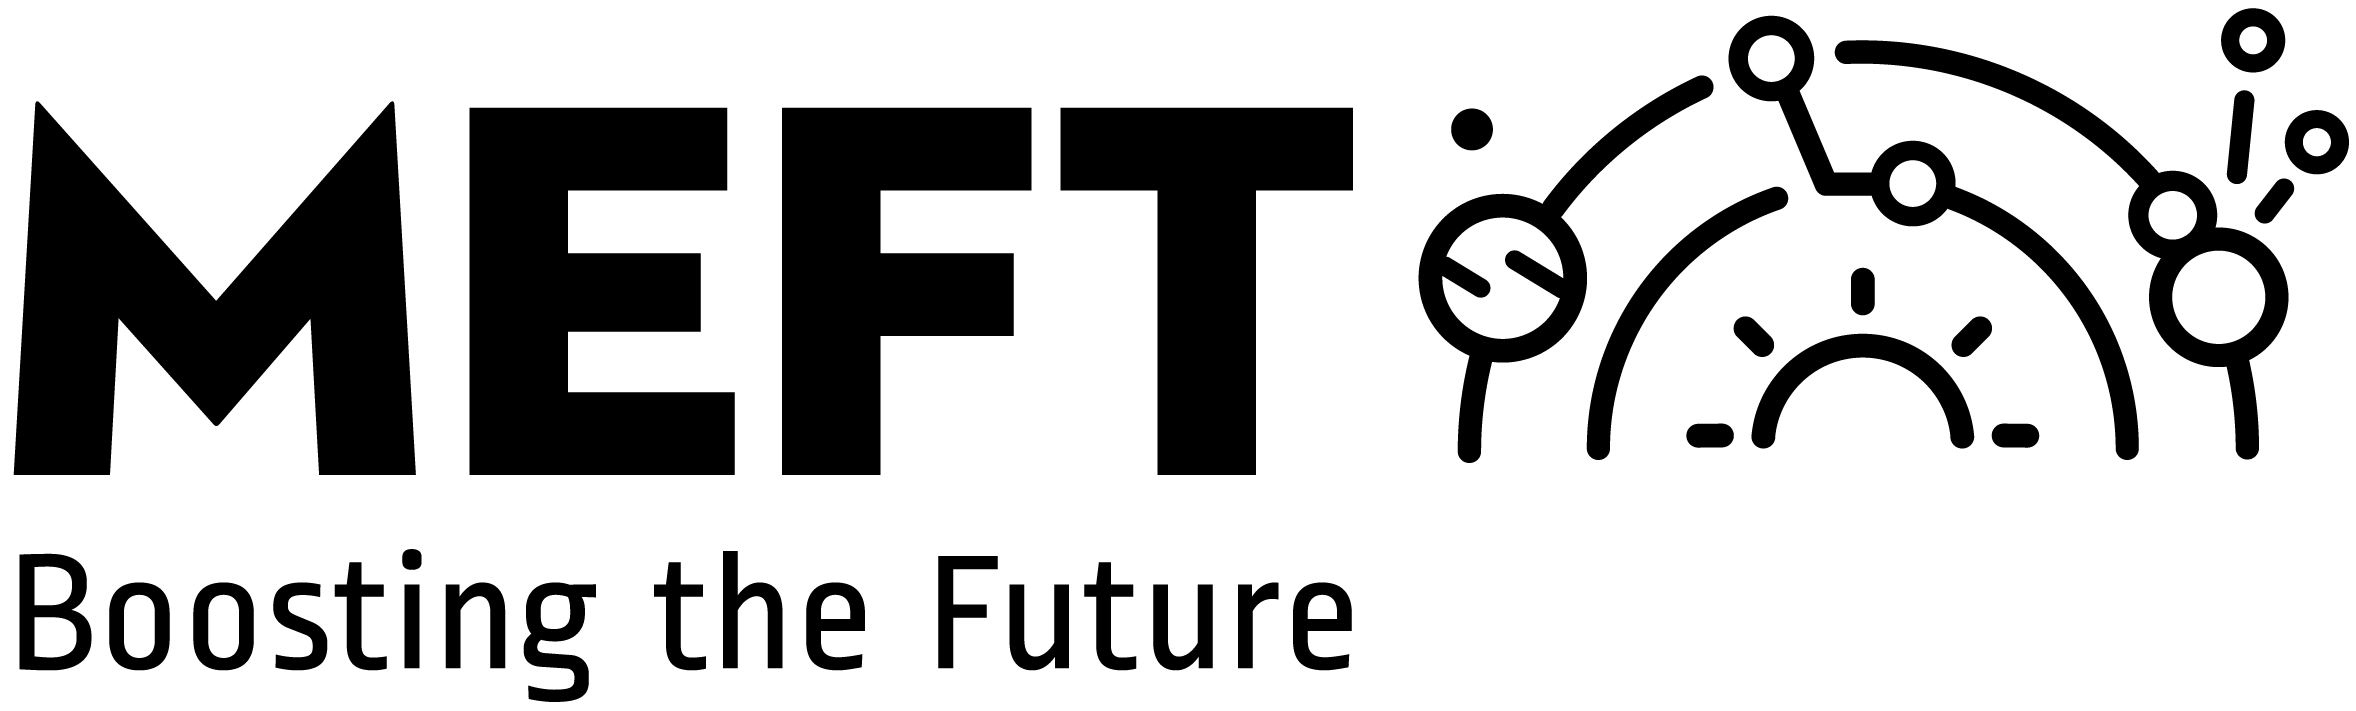
\includegraphics[scale=0.08]{Logo-MEFT_Hor.png}
\end{flushright}
\end{minipage}

\begin{center}

\vspace*{.06\textheight}
{\scshape\LARGE \univname\par}\vspace{1.5cm} % University name
\textsc{\Large Projecto MEFT}\\[0.5cm] % Thesis type

\HRule \\[0.4cm] % Horizontal line
{\huge \bfseries \ttitle\par}\vspace{0.4cm} % Thesis title
\HRule \\[1.5cm] % Horizontal line
 
\begin{minipage}[t]{0.4\textwidth}
\begin{flushleft} \large
\emph{Author:}\\
\href{https://en.wikipedia.org/wiki/Ludwig_Boltzmann}{\authorname} % Author name - remove the \href bracket to remove the link
\end{flushleft}
\end{minipage}
\begin{minipage}[t]{0.4\textwidth}
\begin{flushright} \large
\emph{Supervisor:} \\
\href{https://en.wikipedia.org/wiki/Josef_Stefan}{\supname} % Supervisor name - remove the \href bracket to remove the link  
\end{flushright}
\end{minipage}\\[3cm]
 
\vfill

\large \textit{Research work performed for the \degreename}\\[0.3cm] % University requirement text
\textit{at}\\[0.4cm]
\groupname\\\deptname\\[2cm] % Research group name and department name
 
\vfill

{\small \today}\\[4cm] % Date
%\includegraphics{Logo} % University/department logo - uncomment to place it
 
\vfill
\end{center}
\end{titlepage}


%----------------------------------------------------------------------------------------
%	THESIS CONTENT - CHAPTERS
%----------------------------------------------------------------------------------------

\pagestyle{review} 


%----------------------------------------------------------------------------------------
%	SECTION 1
%----------------------------------------------------------------------------------------
%
%\textcolor{red}{ Homogenise language: use consitently either:
  %null-infinity or null infinity through out (these I've seen a couple
  %of them not consistent, either way is fine but just one way though
  %out the report). Same comment with space-time or spacetime (in
  %english spacetime is ``modern'' way to write it. In spanish and
  %portuguese I think espaço-tempo/espacio-tiempo is standard but in
  %english space-time is a bit old fashioned.)  Also I made some small
  %edits to the text. Please when you re-read the whole document to see
  %them, make sure to homgenise the spelling to be full english or full
  %american. Either way is fine.}%

%\medskip

%\textcolor{red}{ To tidy-up the .tex: Justify inside the text inside
 % .tex file as well.  In emacs it is simply selecting the text and
  %making cntrl + Q.  I've done this in parts of this document so you
  %see how a clean .tex should look inside.}

%\medskip

%\textcolor{red}{Also using two backslashes is not needed. It is enough
 % to leave a black space (line) inside the .tex
  %and if you want more space use skip, medskip
  %or bigskip}

%\medskip

%\textcolor{red}{The equations are not appropriately cited using the
 % .tex commands label and eqref.  You'll see an example inside the
  %.tex. Make this modification through out.}


\begin{justify}
\section{Introduction}
General relativity is a theory of gravitation developed by Albert
Einstein that describes the force of gravity as a curvature of
spacetime caused by mass and energy. In this theory, the force of
gravity is not a force at all, but rather an effect of the way objects
move through spacetime. In general relativity, the presence of a black
hole causes the spacetime around it to bend and curve, resulting in
strange effects such as time dilation and the deflection of light.  A
black hole, seen from an observer that is far away, is similar to a
classical particle and is characterized by three quantities: total
mass, electrical charge and spin. Given the fact that different black
holes which have the same properties are identical, no measurements
can be made to distinguish them \cite{HawMalStr16}.
'Hair' will be
the term which refers to features that help us to tell objects
apart, thus black holes have almost none (No 'hair' theorem). To
understand this theorem on how different objects interact with a black
hole we need to look at the conservation laws, which black holes
obey. When an object falls into a black hole, through conservation we
are able to measure the initial and final black hole to deduce a few
properties the object had. This has important consequences on how
information is handled. Imagine stars and planets of all shapes and
sizes, a black hole would reduce them to only three numbers, meaning
plenty of information is lost. This is a problem known as the
\textit{information paradox} \cite{HawMalStr16}. If a black hole gives
no information on its consumption and then vanishes, then the final
state would be completely independent of the initial state.
In order
to explain this, a recent theory was proposed - soft 'hair'-
corresponding to non-trivial distortions in clocks that is sensitive
to the consumption history of the black hole. Since every possible
orientation of the distant rulers and clocks measure a different soft
hair, in principle there are an infinite amount of properties, where
the notion of distant can be idealised as infinity.
For general relativity, the definition of infinity is complicated as it has to
surpass the ambiguity when discussing coordinate dependent notions and
because there exist different types of infinities. In these report we
will focus on only two types: null-infinity denoted by $\mathscr{I}^+$
and spatial infinity denoted by the symbol $i^0$.
\end{justify}
%%%%
%%% Stylistic advice: avoid small paragraphs
%%%


%-----------------------------------
%	SUBSECTION 1
%-----------------------------------
\subsection{Newman-Penrose constants}
The Newman-Penrose constants ---originally introduced in
\cite{NewPen68}--- are quantities defined on null-infinity. Such
constants obey conservation laws for asymptotically flat
gravitational fields. In flat spacetime, an infinite amount of those
mentioned conservation laws exist for each spin value.
%%
%%\\
%%
For an
isolated system in ordinary Electromagnetic (EM) theory, spin-1 field,
the total charge is conserved, whereas in the linearized gravitational
theory, spin-2 field, the total mass, linear and angular momentum are
also conserved. In this case, we will study, spin-0 fields, which refer
to solutions to the wave equation.  The NP constants form an infinite hierarchy of
conserved quantities for linear equations like the spin-1, spin-2, and
spin-0 fields. Originally, Newman and Penrose showed that such
constants have the form of:
$$G_m = (dipole)^2 - (monopole) \times (quadrupole)$$ ---see
\cite{DaiVal02}.  In the full non-linear gravitational theory, the
mass and momentum are no longer conserved, giving rise to ten
different conserved quantities. It has been discussed whether the NP
constants are zero for stationary spacetimes or not. For the Kerr
solution they are zero \cite{Bac10}, \cite{BaiZhoGonXueXiaoLau07},
which also happens for the Schwarzschild spacetime.
%%%%
%%\\
%%%%
In particular,
it is argued that the magnitude of the constants gives information
about the amount of residual radiation that is contained in the
space-time after a black hole collision \cite{DaiVal02}.  NP constants
retain their value along null-infinity, and as a result of this one
may be able to find information about the final time behaviour of the
process of black hole collision.
%%%
%%\\
%%
Therefore, the Newman-Penrose
constants provide insights into how the system behaves at later times
\cite{DaiVal02}.

%-----------------------------------
%	SUBSECTION 2
%-----------------------------------

\subsection{Friedrich cylinder at spatial infinity}
Roger Penrose brought to the field of general relativity the notion of
conformal transformation, which made a significant impact in the
geometric understanding of infinity. This was crucial for the
development of theory of asymptotics and gravitational radiation,
taking a step forward in the mathematical understanding of
gravitational waves.  Although, customary in numerical approaches to
general relativity, wave forms are computed at large radius, from
first principles point of view they should be computed at null
infinity  $\mathscr{I}^+$. To do
so, the Einstein field equations need to be expressed in terms of
suitably rescaled fields, so one can evaluate the fields at
$\mathscr{I}^+$. Technically this is done by a conformal
transformation. In general relativity, conformal transformations are
used to describe the behavior of physical systems under changes in the
scale of spacetime. These transformations preserve the local structure
of spacetime, but not necessarily its overall shape.
%%%%
%%\\
%%%%
The original
metric, which we refer to as the physical metric, is denoted by
$\tilde{g}$. We consider a transformation to an unphysical metric,
$g$, which is given by
\begin{equation}\label{eq:conftrans}
	g_{ab} = \Xi^2 \tilde{g}_{ab},
\end{equation}
$\Xi$ is a smooth function that approaches zero as the distance from
the source increases. This transformation, denoted by \eqref{eq:conftrans}, preserves
angles, making it appropriate to describe it as conformal.
H. Friedrich introduced the \textit{conformal Einstein field
  equations} (CEFE), a formulation designed that is in accordance with
the approach of R. Penrose.
%%%
%%\\
%%%%%%%%%%%%%%%%%%%%%%%%%%%%%%%%%%%%%%%%%%%%%%%%%%%%%%%%%%%%%%%%%%%%%%%
%%%% Rafael; this a good example of where a space is actually needed.
%%%  the code \\ is not needed. Simply add a space and it will work.
%%%  if you want to add more space use \skip, \medskip, \bigskip
%%%%%%%%%%%%%%%%%%%%%%%%%%%%%%%%%%%%%%%%%%%%%%%%%%%%%%%%%%%%%%%%%%%%%%

\medskip

A prototypical example is the conformal extension of the Minkowski
spacetime which will be discussed in the following.  One starts with
the Minkowski metric line-element,
\begin{equation}\label{eq:metricMink-tr}
	d \tilde{s}^2=-d \tilde{t}^2+d \tilde{r}^2+\tilde{r}^2 d
        \Omega^2,
\end{equation}
where $(\tilde{t}, \tilde{r})$ $\in$ $(-\infty,+\infty)
\times[0,+\infty)$ and $d \Omega^2$ represents the standard metric on
  $\mathbb{S}^2$. To get a conformal extension we need to do a
  coordinate transformation, corresponding to the advance and retarded  
  times, $\tilde{u}=\tilde{t}-\tilde{r}$ $\&$ $\tilde{v}=\tilde{t}+\tilde{r}$,
  %%%%%%%%%%%%%%%%%%%%%
  %%  substituting in (2),
  %%%%%%%%%%%%%%%%%%%%%%%%%%%%%%%%%%%%%%%
  %%%% This is not the appropriate way to cite equations
  %% because if you change the text later and add more equations, what
  %% used to be equation (2) maybe now is equation  (3)
  %% they way to do it is use \label{my-favourite-equation} and \eqref{my-favourite-equation}
  %%%%%%%%%%%%%%%%%%%%%%%%%%%
  substituting equation \eqref{eq:metricMink-tr}.
  %%%%%%%%%%%%%%%%%%%%%%%%%%%%%%
  %\textcolor{red}{The way the equations are cited is not the ``appropriate one'' one
   % uses ``label'' and ``eqref'' for that. Here inside the .tex file you have an example
  %of how to do it. Please do this through out all the report.}
  %%%%%%%%%%%%%%%%%%%%%%%%%%%%%%%
\begin{equation}\label{eq:metricMink-tr1}
	d \tilde{s}^2=-d \tilde{u} d \tilde{v}+\frac{(\tilde{u}-\tilde{v})^2}{4} d \Omega^2.
\end{equation}
For the compactification, we need to introduce the following: $u =
\tan U$ $\&$ $v = \tan V$, where $U$, $V$ $\in$ $(- \pi/2,
\pi/2)$. Now, we are able to identify the conformal metric,
$ds$. Using \eqref{eq:metricMink-tr}, we obtain
$$d s^2=-4 d U d V+\sin ^2(V-U) d \Omega^2$$ where
$$d s^2=\Xi^2 d \tilde{s}^2$$ with $\Xi=2 \cos U \cos V$. Given the
domain of $U$ and $V$, we introduce the following, $T=V+U$ $\&$
$\psi=V-U$. The domain of $(T, \psi)$ is $(-\pi, \pi)$, with
\begin{equation}\label{eq:metricMink-cf}
	d s^2=-d T^2+d \psi^2+\sin ^2 \psi d \Omega^2,
\end{equation}
where we define this as the standard Lorentzian metric on $\mathbb{R}
\times \mathbb{S}^3$ or the Einstein Cylinder.
%%%%%
%%\\
%%%%
The purpose of this report is to study what happens at infinity, and
in order to do that we will focus on the region where $\Xi = 0$. This
condition gives us the following regions, which are presented in the
following table
%\textcolor{red}{put some headings to the columns. Make the table with
 % three columns with headings: Region/ Name/ Symbol. }
\begin{center}
\begin{tabular}{ |c|c|c| }
  \hline
  Region & Name & Symbol \\
 \hline
 $\tilde{r} \rightarrow \infty \enspace \;  \text{with} \; \;\;\;\;
 |\tilde{t}| $<$ \infty$ & Spatial Infinity & $i^{0}$ \\
 \hline 
 $\tilde{t} \rightarrow \pm \infty$  \;\; with \;\; $\tilde{r}$<$\infty$
 \enspace & Future/Past Timelike Infinity & $i^{\pm}$ \\
 \hline
 $\tilde{r} \rightarrow \infty, \enspace \tilde{t} \rightarrow \infty \enspace
 \text{with} \;\; |u|$<$\infty$ &  Future Null-infinity & $\mathscr{I}^+$ \\ 
 \hline
 $\tilde{r} \rightarrow\infty, \enspace \tilde{t} \rightarrow-\infty \;\;
 \text{with} \enspace |v|$<$\infty$ & Past Null-infinity & $\mathscr{I}^-$ \\
 \hline
\end{tabular}
\end{center}
The visual representation of this is a Penrose Diagram, depicted in
Fig.1
\begin{figure}[h]
	\centering 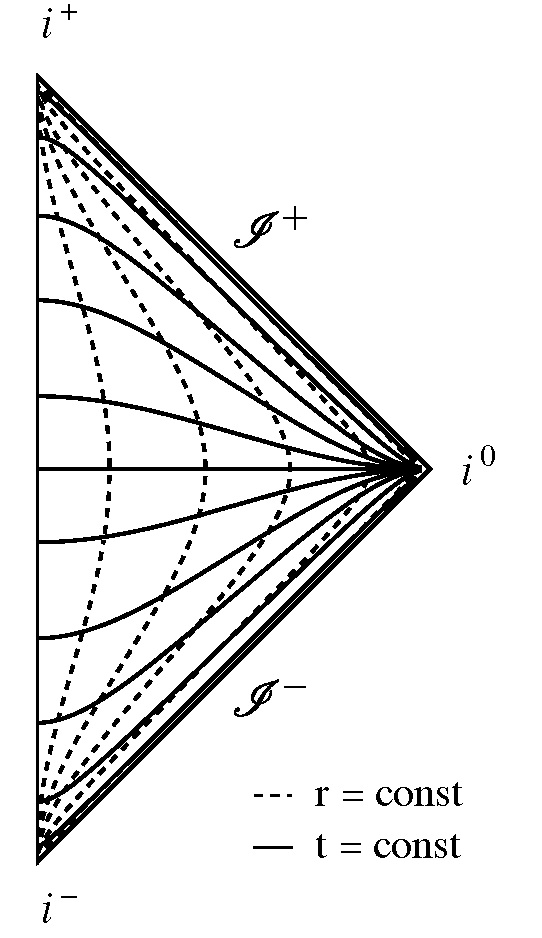
\includegraphics[width =0.25\textwidth]{Penrose diagram.pdf}
    \caption{Penrose Diagram - Representation of the standard
      compactification of the Minkowski spacetime alongside the curves of constant
      time, solid black lines, and the curves of constant r, dotted
      black lines.}
\end{figure}
Additionally, H. Friedrich proposed another conformal
representation of Minkowski spacetime specifically adapted for
spatial infinity, which will be the one used in this work. By applying
the following change of coordinates $\tilde{t} =
\frac{\tau}{\rho(1-\tau^{2})}$, \enspace $\tilde{\rho} =
\frac{1}{\rho(1-\tau^{2})}$ we arrive at this representation.
Therefore,
$$ \gamma=-d \tau^2+\frac{\left(1-\tau^2\right)}{\rho^2} d
\rho^2-\frac{\tau}{\rho}(d \rho d \tau+d \tau d \rho)+d \Omega^2 $$ We
are now in the position to say that the conformal factor $\Theta$ is
given by,
\begin{equation}\label{eq:gamma}
	\gamma = \Theta^2 \tilde{\eta}.
\end{equation}
\begin{equation}\label{eq:conf-factor}
	\Theta = \rho(1-\tau^2).
\end{equation}

\begin{figure}
	\centering
    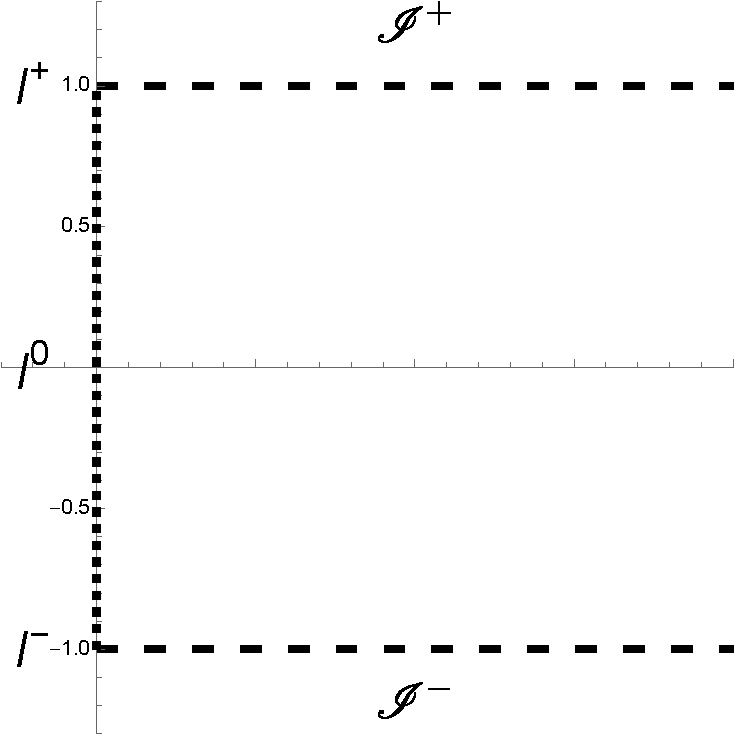
\includegraphics[width =0.3\textwidth]{friedrich cylinder.pdf}
    \caption{Representation of the Friedrich Cylinder. Past null infinity is represented by $\mathscr{I}^-$, Future null infinity as $\mathscr{I}^+$, spatial infinity as $I^{0}$ and the critical sets as $I^{+}$ and $I^{-}$.}
\end{figure}

As a result of the spacetime admitting only particles that travel
slower than the speed of light, which in geometric units corresponds to $\pm 1$,
hence, we have
%%%%
%% than $c$, we have,
%% c wasn't defined. Better to write speed of light.
%%%
$$ -1 \le \tau \le 1 $$ with $\rho$ > 0. Therefore, light travels towards infinity to
the places where $\tau = \pm 1$ in the conformal extension. So, in this representation,
$$ \mathscr{I}^+ \equiv \{ \tau = 1 \}, \enspace \mathscr{I}^- \equiv
\{ \tau = -1 \}$$ The sets where future and past null-infinities touch
spatial infinity are named the critical sets and are given by,

$$ \mathcal{I}^+ = \{ \tau = 1, \enspace \rho = 0\}, \enspace
\mathcal{I}^- = \{ \tau = -1, \enspace \rho = 0\}$$
%----------------------------------------------------------------------------------------
%	SECTION 2
%----------------------------------------------------------------------------------------

\section{NP - constants for spin-0 fields close to $i^{0}$ \& $\mathscr{I}^+$ in flat spacetime}
The $i^0$ cylinder representation has previously been used to
calculate the NP constants for the spin-1 and spin-2 fields in flat
space in \cite{ValKro02gb} and \cite{GasKro16d}. In this report, we
will perform a similar analysis for the solution to the wave equation,
or spin-0 field. This calculation represents an extension of the
analysis of linear fields propagating near spatial and null-infinity
in flat spacetime.  We are now in the position to calculate the
Newman-Penrose constants for spin-0 fields, and by spin-0 fields
we mean the wave equation. Therefore, the Newman-Penrose constants for
the wave equation are obtained in the following way.
%%\\
%%%
First, we need to introduce the solution to the wave equation in
Minkowski spacetime,

\begin{equation}\label{eq:wave-eq}
	\tilde{\Box} \tilde{\phi} = 0.
\end{equation}
Following we need to introduce the radiation field, denoted by $\psi =
\tilde{\rho}\tilde{\phi}$ and \eqref{eq:wave-eq} reads as follows,

\begin{equation}\label{eq:wave-eq-rewriten}
	\partial_{\tilde{u}}\partial_{\tilde{v}}\psi =
        \frac{1}{\tilde{\rho}^2}\Delta_{\mathbb{S}^2}\psi,
\end{equation}
where we have that $\partial_{\tilde{v}} = \partial_{\tilde{t}} +
\partial_{\tilde{\rho}}$ \& $\partial_{\tilde{u}} =
\partial_{\tilde{t}} - \partial_{\tilde{\rho}}$ and
$\Delta_{\mathbb{S}^2}$ being the Laplacian on $\mathbb{S}^2$.\\ It is
of great advantage to make a harmonic decomposition, such that $\psi =
\sum_{l = 0}^{\infty}\sum_{m = -l}^{l}\psi_{lm}Y_{lm}$ and
$\Delta_{\mathbb{S}^2}Y_{lm} = -l(l+1)$. As a result \eqref{eq:wave-eq-rewriten} reads:

\begin{equation}\label{eq:wave-eq-harmDecomp}
	\partial_{\tilde{u}}\partial_{\tilde{v}}\psi_{lm} =
        \frac{-l(l+1)}{\tilde{\rho}^2}\psi_{lm},
\end{equation}
\\ And \eqref{eq:wave-eq-harmDecomp} implies that \cite{GajKehLeo22}

$$\partial_{\tilde{u}}(\tilde{\rho}^{-2l-2}(\tilde{\rho}^2\partial_{\tilde{v}})^{l+1}\psi_{lm})
= 0, \enspace
\partial_{\tilde{v}}(\tilde{\rho}^{-2l-2}(\tilde{\rho}^2\partial_{\tilde{u}})^{l+1}\psi_{lm})
= 0$$ \\ The higher-order NP-constants for (7) are defined at
$\mathscr{I}^+$ \cite{Keh21},
$$\mathcal{I}^+_{lm} = \lim_{\tilde{v} \to \infty}
\tilde{\rho}^{-2}\partial_{\tilde{v}}((\tilde{\rho}^2\partial_{\tilde{v}})^{l}\psi_{lm})$$
Our goal is to use conformal methods and the framework of the cylinder
at spatial infinity to compute $\mathcal{I}^+_{lm}$. To do this, we need
to recall that for two conformally related manifolds - which do not
necessarily have to be the $i^0$ cylinder and Minkowski spacetime -
$(\tilde{M},\tilde{g})$ and $(M,g)$, the D'Alembertian operator
transforms under conformal transformations as follows
\cite{DuaFenGasHil22}:

\begin{equation}\label{eq:waveConfTr}
	\square \phi-\frac{1}{6} \phi R=\Theta^{-3}\left(\tilde{\square} \tilde{\phi}-\frac{1}{6} \tilde{\phi} \tilde{R}\right),
\end{equation}
where $R$ and $\tilde{R}$ are the Ricci scalars of $g$ and $\tilde{g}$ respectively and $\phi = \Theta^{-1}\tilde{\phi}$.
%%%%%%%
%%%
%%\\
%%\\
%%%%%%

\bigskip

By applying the conformal transformation formula for the wave equation, given in equation \eqref{eq:waveConfTr}, to the wave equation in \eqref{eq:wave-eq} on the physical Minkowski spacetime $(\tilde{M} , \tilde{\eta})$ and selecting the target conformal extension - the unphysical spacetime - $(M, g)$ to be Friedrich's cylinder at spatial infinity, we can obtain the following equation:

\begin{equation}\label{eq:wave-unphysical}
	\square \phi = 0.
\end{equation}
Thus, \eqref{eq:wave-unphysical} is just the wave equation for the unphysical field propagating on the $i^0$ cylinder background.
%%\\
%%\\

\medskip

A calculation shows that the conformal factor, in terms of physical
coordinates is given simply by the inverse of the physical polar
coordinate, additionally, further calculations show that:
$$\Theta^{-1} = \tilde{\rho}^{-1} \implies \phi =
\tilde{\rho}\tilde{\phi} \implies \psi = \phi$$
$$ \textit{L} := \partial_{\tilde{v}}, \enspace
\underbar{\textit{L}}:= \partial_{\tilde{u}}, \enspace L =
k^{-1}\Theta l, \enspace \underbar{\textit{L}} = k\Theta l$$ where $l
= (1+\tau)\partial_{\tau}-\rho \partial_{\rho}$,
$\underbar{\textit{l}} = (1-\tau)\partial_{\tau}+\rho
\partial_{\rho}$ and $k = \frac{(1+\tau)}{(1-\tau)}$.  To compute the NP constants, the following rescaled
null derivative will play an important role $\hat{L}:=
\tilde{\rho}^2L$ which explicitly reads
\begin{equation}\label{eq:operator}
  \hat{L} = \rho^{-1}(1+\tau)^{-1}\partial_{\tau} -
  (1+\tau)^{-2}\partial_{\rho}.
\end{equation}
One can translate the expression above for the NP constants given
above to the ones as follows,
$$l = 0 \rightarrow \tilde{\rho}^2L\phi_{00} \rightarrow
\hat{L^{1}}\phi_{00} = \langle \hat{L^1}\phi,Y_{00}\rangle,$$
$$l = 1 \rightarrow (\tilde{\rho}^2L)^2\phi_{1m} \rightarrow
\hat{L^{2}}\phi_{1m} = \langle \hat{L^2}\phi,Y_{1m}\rangle,$$
$$l = l \rightarrow (\tilde{\rho}^2L)^{l+1}\phi_{lm} \rightarrow
\hat{L}^{l+1}\phi_{lm} = \langle \hat{L}^{l+1}\phi,Y_{lm}\rangle,$$
where the symbol $\langle,\rangle$ represents the inner-product defined as
\begin{align}\label{innerprod}
  \langle \alpha, \beta \rangle = \frac{1}{4\pi}\int_0^{2\pi}\int_0^\pi \alpha \beta \sin(\theta)d\theta d\phi,
\end{align}
%\textcolor{red}{I could write it, but I want you to think what it is to make sure you
%understand what the notation actually represents.}
where $\alpha$ and $\beta$ are functions of the coordinates spacetime coordinates.
The orthogonality property of the spherical harmonics in this notation reads
$\langle Y_{lm}, Y_{l'm'}\rangle = \delta_{ll'}\delta_{mm'}$.
%%%%
%%% $\langle\phi, Y_{lm}\rangle$ refers to the integration over the
%%% spherical harmonics.
%%\\
%%%%
Following \cite{MinMacKro22}, we take as Ansatz for the solution to
the wave equation:

\begin{equation}\label{eq:ansatz}
	\phi = \sum_{p = 0}^{\infty}\sum_{l = 0}^{p}\sum_{m = -l}^{m =
          l}\frac{1}{p!}a_{p;l,m}(\tau)\rho^{p}Y_{lm}.
\end{equation}
%%\\
Then, a calculation using the orthogonality of the spherical
harmonics gives:
\begin{equation}\label{ansatz-1}
	\phi_{lm} = \langle\phi, Y_{lm}\rangle = \sum_{p =
          0}^{\infty}\frac{1}{p!}a_{p;l,m}(\tau)\rho^p .
\end{equation}
%%%%%%%%% This is not needed if the general expression is given above
%%%%%%%%%%
%%%\\ where $\langle\phi, Y_{lm}\rangle = \int_{\mathbb{S}^2} \sum_{p =
%%  0}^{\infty}\sum_{l' = 0}^{p}\sum_{m' =
%%  -l'}^{l'}\frac{1}{p!}a_{p;l',m'}(\tau)\rho^{p}Y_{l'm'}Y_{lm}
%%\,d\mathbb{S}$
%%%%%%%%%%%%%%
%%\\
Equation \eqref{eq:wave-unphysical} was solved in \cite{MinMacKro22} and the solution is
encoded in the following lemma.
\begin{lemma} (Minucci, Panosso Macedo \& Valiente Kroon 2022 \cite{MinMacKro22})
	\begin{enumerate}
	\item For $p\geq 1$ and $0\leq \ell \leq p-1$
	 \begin{align}\label{eq:lemma1-1}
    a(\tau)_{p;\ell,m} =A_{p,\ell,m}
		  \bigg(\frac{1-\tau}{2}\bigg)^{p}
                  P_{\ell}^{(p,-p)}(\tau) + B_{p,\ell,m}
                  \bigg(\frac{1+\tau}{2}\bigg)^{p}P_{\ell}^{(-p,p)}(\tau)
	 \end{align}
	
	\item For $p\geq 0$ and $\ell=p$:
     \begin{align}\label{eq:lemma1-2}
      {a}_{p;p,m}(\tau) =
      \bigg(\frac{1-\tau}{2}\bigg)^{p}\bigg(\frac{1+\tau}{2}\bigg)^{p}\Bigg(C_{p,p,m}
      +D_{p,p,m}\int_{0}^{\tau} \frac{ds}{(1-s^2)^{p+1}}\Bigg)
     \end{align}
	where $A_{p,\ell,m}$, $B_{p,\ell,m}$, $C_{p,p,m}$ and
        $D_{p,p,m}$ are constants that can be written in terms of
        $a_{p;\ell,m}(0)$ and $\dot{a}_{p;\ell,m}(0)$ and
        $P_{\gamma}^{\alpha, \beta}(\tau)$ are the Jacobi polynomials.
    \end{enumerate}
\end{lemma}

Expanding the integral in \eqref{eq:lemma1-2} results in logarithmic terms, hence
$D_{p,p,m} = 0$ is called the regularity condition. The solutions for
$a(\tau)$ are polynomic in $\tau$, except for $l = p$ where one needs
to impose the regularity condition to only have polynomic
solutions. \cite{MinMacKro22}.  \\ \\ Using the following notation:
$$\Lambda^2 := \Theta^{-1}k^{-1} = \rho^{-1}(1+\tau)^{-2}, \enspace e
:= (1+\tau)\partial_{\tau} - \rho\partial_{\rho}$$ \\ we can rewrite
the operator $\hat{L}$ as $\hat{L} = \Lambda^2 e$. Applying $\hat{L}$
to our scalar field one gets that
$$\hat{L}\phi = \Lambda^2\sum_{p,l,m}^{}Y_{l,m}\rho^{p}
[(1+\tau)\dot{a}_{p;l,m}-pa_{p;l,m}]$$ where
$(1+\tau)\dot{a}_{p;l,m}-pa_{p;l,m} = A^{0}_{p;l,m}(\tau)$ and $\sum_{p,l,m} = \sum_{p = 0}^{\infty}\sum_{l = 0}^{p}\sum_{m = -l}^{m =
l}$\\ The
general formula to compute the NP constants is given by,

$$\mathcal{I}^+_{lm} = \lim_{\substack{\rho \to 0 \\ \tau \to 1}}
\langle\hat{L}^{l+1}\phi, Y_{lm}\rangle$$\\ The NP constant is being
evaluated at the critical set $\mathcal{I}^+$, hence $\rho =
0, \enspace \tau = 1$.  We are now able to calculate the first NP
constant, which is the case where $l = 0$. Thus, we have,

$$\mathcal{I}^+_{0m} = \lim_{\substack{\rho \to 0 \\ \tau \to 1}} \langle\hat{L}\phi, Y_{00}\rangle = \lim_{\rho \to 0}\sum_{p = 0}^{\infty}\frac{1}{p!}2^{-2}\rho^{p-1}A^{0}_{p,0,0}(1)$$
$$ \Leftrightarrow \mathcal{I}^+_{0m} = \lim_{\rho \to 0} \biggl\{ \frac{2^{-2}}{0!}\rho^{-1}A^0_{0,0,0}(1)+\frac{2^{-2}}{1!}A^0_{1,0,0}(1) \biggr\}$$
Now, we want to evaluate $A^0_{p,l,m}$:\\
$$A^0_{p;l,m}(\tau) = (1+\tau)\dot{a}_{p;l,m}(\tau)-pa_{p;l,m}(\tau) \rightarrow 2\dot{a}_{0,0,0}(\tau) = \frac{-D_{0,0,0}}{\tau - 1}$$
$$A^0_{1,0,0}(\tau) = 2\dot{a}_{1,0,0}(\tau) - 1 \times a_{1,0,0}(\tau) = - A_{1,0,0}$$Imposing the regularity condition: 
$$D_{0,0,0} = 0 \rightarrow \mathcal{I}^+_{0m} = \frac{-A_{100}}{4}$$\\
Being $A_{100}$ determined by initial data as read from Lemma 1. To determine NP constants with $l = 1$, one needs to compute:

$$\mathcal{I}^+_{1m} = \lim_{\substack{\rho \to 0 \\ \tau \to 1}} \langle\hat{L}^2\phi, Y_{1m}\rangle$$
The expression for $\hat{L}^2\phi$ is given by,
$$\hat{L}^2\phi = \Lambda^4 \sum_{p,l,m}Y_{lm}\rho^p[(1+\tau)\dot{A}^0_{p;l,m} - (p+1)A^0_{p;l,m}]$$
where,
$$A^1_{p;l,m} = (1+\tau)\dot{A}^0_{p;l,m} - (p+1)A^0_{p;l,m}$$
Thus,
$$\mathcal{I}^+_{1m} = \lim_{\substack{\rho \to 0 \\ \tau \to 1}}2^{-4} \{\rho^{-2}A^1_{0,1,m}(\tau) + \rho^{-1}A^1_{1,1,m}(\tau)\} + \lim_{\rho \to 0} 2^{-4}\frac{1}{2!}A^1_{2,1,m}(\tau)$$
Evaluating $A^1_{p;l,m}$ and imposing the regularity condition, one finds that the NP constant for $l = 1$ is given by,
$$\mathcal{I}^+_{1m} = 2^{-4} \frac{1}{2!}6A_{211}$$
\\
The previous discussion suggests that, in principle, it should be possible to obtain a general formula $A_{p;l,m}(\tau)$. Revising the calculation of $\mathcal{I}^+_{0m}$ and $\mathcal{I}^+_{1m}$ one can obtain the following results concerning the overall structure of the spin-0 NP constants.
\\
We start with,
$$A^n = k_0\binom{n+1}{0}(1+\tau)^n a^{(n)} - k_1\binom{n+1}{1}p(1+\tau)^{n-1}a^{(n-1)}+...+(-1)^n\binom{n+1}{q}k_q a$$
where $a^{(n)}$ is the $n-th$ derivative, $A^{n}$ is shorthand for $A^{n}_{p,l,m}$ and we define $k_q$ to be,
$$k_q := \frac{p(p+q-1)!}{p!}$$
\\
Therefore,

\begin{equation}\label{eq:A^n}
	A^n_{p,l,m} = \sum_{q=0}^{n+1}(-1)^q\frac{(p+q-1)!}{(p-1)!}\binom{n+1}{q}(1+\tau)^{n-q+1}a^{(n-q+1)}.
\end{equation}
\\
The following lemma will be proved.
\begin{lemma} [Gasper\'in $\&$ Pinto 2023]
\begin{equation}\label{eq:lemma2-1}
	\hat{L}^n \phi = \Lambda^{2n}\sum_{p = 0}^{\infty}\sum_{l = 0}^{p}\sum_{m = -l}^{m = l}\frac{1}{p!}\rho^{p}A^{n-1}_{p,l,m}(\tau)Y_{0,l,m},
\end{equation}
\end{lemma}
with,
\begin{equation}\label{eq:lemma2-2}
	A^{n-1}_{p,l,m} = \sum_{q=0}^{n}(-1)^q k_q \binom{n}{q}(1+\tau)^{n-q} a^{(n-q)}.
\end{equation}
\\
Proof:\\
The basis of induction for arriving at the general formula for the NP constants will be the cases $n=0$ and $n=1$ and the induction hypothesis will be \eqref{eq:lemma2-1} and \eqref{eq:lemma2-2}. The induction step is as follows,
$$\hat{L}^{n+1}\phi = \hat{L}(\hat{L}^n\phi) = \Lambda^{2(n+1)}\sum_{p,l,m}Y_{lm}\rho^p[(1+\tau)\dot{A}^{n-1}_{plm}-(p+n)A^{n-1}_{plm}]$$
\\
Thus we have shown that,
$$\hat{L}^{n+1}\phi = \Lambda^{2(n+1)}\sum_{p,l,m}Y_{lm}\rho^p R^n_{plm}$$
where
$$R^n_{plm} := (1+\tau)\dot{A}^{n-1}_{plm}-(p+n)A^{n-1}_{plm}$$
Using the induction hypothesis \eqref{eq:lemma2-2} we can compute all the pieces to construct $R^n_{plm}$:
\begin{equation}\label{eq:lemma2-3}
	R^{n}_{plm} = \sum_{q=0}^{n}(-1)^q k_q \binom{n}{q}\{(1+\tau)^{n-q+1} a^{(n-q+1)} - (p+q)(1+\tau)^{n-q} a^{(n-q)}\}.
\end{equation}
\\
Expanding the first term in the first sum of \eqref{eq:lemma2-3} renders
$$R^{n}_{plm} = (-1)^0 k_0 \binom{n}{0}(1+\tau)^{n+1} a^{(n+1)} + \sum_{q=1}^{0}(-1)^q k_q \binom{n}{q}(1+\tau)^{n-q+1} a^{(n-q+1)} - $$
$$-\sum_{q=0}^{n}(-1)^q k_q \binom{n}{q}(p+q)(1+\tau)^{n-q} a^{(n-q)}$$
Separating the last term in the second sum and rearranging gives
$$R^{n}_{plm} = k_0(1+\tau)^{n+1}a^{(n+1)} + \sum_{q=1}^{n}(-1)^q k_q \binom{n}{q}(1+\tau)^{n-q+1} a^{(n-q+1)} + $$
$$ + \sum_{q=0}^{n-1} \bigg[(-1)^{q+1}k_{q+1}\binom{n}{q}(1+\tau)^{n-q}a^{(n-q)}\bigg] + (-1)^{n+1}k_{n+1}a$$
\\
Relabelling $i = q-1 \implies q = i+1$, \enspace $i(q=1) = 0$ $\&$ $i(q=n+1) = n$
$$R^{n}_{plm} = k_0(1+\tau)^{n+1}a^{(n+1)} + \sum_{i=0}^{n-1}(-1)^{i+1} k_{i+1} \binom{n}{i+1}(1+\tau)^{n-i} a^{(n-i)} + $$
$$ + \sum_{q=0}^{n-1} \bigg[(-1)^{q+1}k_{q+1}\binom{n}{q}(1+\tau)^{n-q}a^{(n-q)} \bigg] + (-1)^{n+1}k_{n+1}a$$
\\
For the second sum we simply relabel the dummy index $i=q$ and get
$$R^{n}_{plm} = k_0(1+\tau)^{n+1}a^{(n+1)} + \sum_{i=0}^{n-1}(-1)^{i+1} k_{i+1} \bigg[\binom{n}{i+1}+\binom{n}{i} \bigg](1+\tau)^{n-i} a^{(n-i)} + (-1)^{n+1}k_{n+1}a$$
\\
Using the recursive identity of the binomial coefficients we get
$$R^{n}_{plm} = \sum_{q=0}^{n+1}(-1)^{q}k_{q}\binom{n+1}{q}(1+\tau)^{n-q+1}a^{(n-q+1)} = A^{n+1}_{plm}$$
\\
Therefore, we have proven that \eqref{eq:A^n} is indeed the general formula for calculating the NP constants. For completeness of this proof, we need to introduce one final lemma,

\begin{lemma}[Gasper\'in $\&$ Pinto 2023]\label{lemma3}
	%%\begin{enumerate}
	\item If the regularity condition is satisfied and the NP constants are finite then they are determined in terms of the initial data by
	 \begin{align}\label{eq:lemma3}
		\mathcal{I}^+_{nm} = Q(n)A_{(n+1),n,m}
	 \end{align}
	where $Q(n)$ is a numerical coefficient $\&$ $A_{(n+1),n,m}$ is determined by the initial data, for $\phi$ on $\tau = 0$.
	%%\end{enumerate}
\end{lemma}

Using Lemma 2, %\textcolor{red}{cite which lemma. Again you can use ``label'' and ``cite'' with lemmas. " label \{my-favourite-lemma\} '' and `` cite \{ my-favourite-lemma \}'' },

$$\mathcal{I}^+_{nm} = \lim_{\substack{\rho \to 0 \\ \tau \to 1}} \langle\hat{L}^{n+1}\phi, Y_{nm}\rangle = \lim_{\substack{\rho \to 0 \\ \tau \to 1}}(1+\tau)^{-4(n+1)}\sum_{p=0}^{\infty}\frac{1}{p!}\rho^{p-2(n+1)}A^{n}_{pnm}(\tau) \Leftrightarrow $$
$$\Leftrightarrow \mathcal{I}^+_{nm} = \frac{2^{-4(n+1)}}{(n+1)!}A^{n}_{n+1,n,m}(\tau)$$
Evaluating $A^{n}_{n+1,n,m}$ at $\tau = 1$, one gets \eqref{eq:lemma3}.
\section{Conclusions and future work}

%\textcolor{red}
 %         {the conclusions are too short. It needs to be a bit longer. At least two paragraphs.
  %One sometimes needs to repeat a bit what was said in the introduction.
  %Imagine it as being a summary of the whole report.}

%\textcolor{red}{Also, maybe, throught use $\mathcal{I}_{nm}^{+}$ to denote these were computed at future null infinity (or better said, the critical set $I^+$) so that when you talk about future work you say that you want to compute $\mathcal{I}_{nm}^{-}$ which are the NP constants at past null infinity..... }
General relativity is a theory of gravitation that explains the force of gravity as a curvature of spacetime caused by mass and energy. Black holes, which are objects with such strong gravitational forces that nothing, not even light, can escape them, are an important aspect of this theory. When an object falls into a black hole, it is reduced to just three numbers, leading to the loss of a large amount of information, a problem known as the "information paradox." A recent theory called "soft hair" has been proposed to explain this paradox by positing that non-trivial distortions in clocks, sensitive to the black hole's consumption history, can provide an infinite number of properties for a black hole in certain limits. The Newman-Penrose (NP) constants are quantities defined on null-infinity in general relativity that obey conservation laws for asymptotically flat gravitational fields. These constants can be used to study the residual radiation present in spacetime after a black hole collision, and have been shown to be zero for stationary spacetimes such as the Schwarzschild and Kerr solutions. However, it is still an open question whether the NP constants are zero for all stationary spacetimes.
\\
 In the future, we want to examine the NP constants of the critical set $\mathcal{I}_{nm}^-$
to see if there is a connection between the NP constants of the past
and those of the future. Calculating the NP constants may allow us to
retrieve the logarithmic solutions obtained through the conformal
method using asymptotic expansions in a physical setting similar to
those described in \cite{DuaFenGas22}.

%%\pagebreak
%----------------------------------------------------------------------------------------
%	BIBLIOGRAPHY
%----------------------------------------------------------------------------------------
\section{Bibliography}




%\bibliographystyle{reporthack}
%\bibliography{refs}

\printbibliography[]

%%%%%%%%%%%%%%%%%%%%%%%%%%%%%%%%%%%%%%%%%%%%%%%%%%%%%%%%%%%%%%%%%%%
%\bibliography{refs}
%%%%%%%%%%%%%%%%%%%%%%%%%%%%%%%%%%%%%%%%%%%%%%%%%%%%%%%%%%%%%%%%%%%

%----------------------------------------------------------------------------------------
\end{document}
